\documentclass[12pt]{article}
\usepackage{fontenc}
\usepackage{mathptmx}
\usepackage{setspace}
\doublespacing
\usepackage{graphicx} % Required for inserting images

\usepackage{natbib}

\usepackage[hybrid,fencedCode]{markdown}
\usepackage{minted}

\usepackage{hyperref}
\hypersetup{
  colorlinks=true, 
  linkcolor=black,
  citecolor=blue,
  urlcolor=blue
}

\usepackage{titlesec}
\titleformat{\subsubsection}[runin]{\normalsize\bfseries}{\thesubsection}{5pt}{}

\usepackage{amssymb, amsfonts, amsmath}
\usepackage{bm}
\usepackage[margin=1.5cm]{geometry} % full-width
    \topskip        =   20pt
    \parskip        =   10pt
    \parindent      =   0 pt
    \baselineskip   =   15pt


\usepackage{adjustbox}              % resizing
\usepackage{caption}                % to reset the cations etc 
\usepackage{rotating}               % for the sidewaystable
    \numberwithin{table}{section}   % reset the Table numbering for each section
\usepackage{booktabs}               % neatly formatting lines
\usepackage{dcolumn}                % aligning decimals
    \newcolumntype{d}[1]{D{.}{.}{#1}}

\newcommand{\sym}[1]{\rlap{#1}} % for the stars

\begin{document}

\begin{titlepage}
    \begin{center}
        \vspace*{1cm}
        {\huge
        Herding within Chinese Equity Markets in Response to COVID-19
’Lockdown Style’ Containment Measures}
        \vspace{0.5cm}
        \\
        {\large By}
        \\
        \vspace{0.5cm}
        \textbf{Sam L. Blundell}
   		\vspace{1.5cm}
        \center{\huge{\textbf{Applied Economic Dissertation}}}
        \\
        \vspace{1.5cm}
       
\includegraphics[scale=1]{TeX_files/bristolcrest_colour.pdf}
    
        \vspace{10mm}
        \large{School of Economics}
        \\
        \textsc{University of Bristol}

        \vspace{0.8cm}

        \large{March 2023}
        
    \end{center}
    
 

\end{titlepage}

\tableofcontents

\break

\section{Introduction}

\break

\section{Theoretical and Empirical Review}

\subsection{Theory of Herding}



\subsection{Empirical Literature Review}

In the 30 years following the seminal article \citet{scharfstein}, 329 articles have been published on the topic of herding in financial markets with 15,900 citations \citep{choijil}. Since the Great Financial Crisis, there has been a significant surge in the number of papers published on the topic, with the majority of them appearing in the last seven years. In fact, the number of articles published and the corresponding citations during this period have surpassed those of the previous 24 years.

This large body of empirical literature covers numerous models of herding, markets, events and herding consequences. However, there still exists significant gaps within this body, most notably to the purposes of this paper including empirical evidence of irrational-based models of herding. The following literature review seeks to provide insights into the empirical work relevant to this paper’s aims, which will inform our subsequent econometric approach and interpretation of empirical results.

\subsubsection*{[Measures of Herding]} 

During his herding in financial markets literature review, \citet{spyrou} splits empirical approaches to measuring herding into two categories - approaches that rely on micro-data or proprietary data, and approaches that rely on aggregate pricing or market data.

The latter approach was pioneered by \citet{ch} (herein referred to as CH), who based their methodology on the observation that if herding is present within a market, the dispersion of returns from the average market return is expected to decrease. This is due to the fact that investors who follow each other’s investment choices will drive individual assets returns towards the mean. CH defines dispersions as the cross-sectional standard deviation of returns:

$$
CSSD=\sqrt{\frac{\sum^n_{i=1}{(r_i-\bar{r})^2}}{n-1}}
$$

where $r_i$ is the individual stock return of stock $i$ and $\bar{r}$ is the cross-sectional average of the $n$ returns within the market portfolio. CH as such suggests that during periods of ‘market stress’, defined as abnormally high or low aggregate market returns, we expect investors are more likely to herd, and thus dispersions will decrease in herding during these periods. They define a regression specification to capture this relationship, 

$$
CSSD_t=\alpha+\beta_1D^L_t+\beta_2D^U_t+\epsilon_t
$$

where $D^L_t$ and $D^U_t$ are binary indicators capturing when market returns fall within the lower and upper tails of the distribution, respectively. Within CH’s regressions, they set these tails both at the 5\% and 1\% criteria arbitrarily. Crucially to the explanatory power of this method, this prediction is is complete contradiction to that of rational asset-pricing models. These models dictate that dispersions will increase as market returns reach the tails of the distribution due to individual assets varying in degrees of sensitivity to overall market returns. As such, significant negative values of $\beta_1$ and $\beta_2$ contradict rational asset-pricing models and indicate herding is present within a market.

CH carries out an analysis of herding within ordinary common shares traded in US equity markets, breaking these shares into industry groups to determine the presence of industry-based herding. CH estimates a significantly positive $\beta_1$ and $\beta_2$ for all industries and overall, indicating herding is not present within the market. This result is consistent when using both daily and monthly data, failing to confirm CH’s hypothesis that the use of daily data may restrict the type of herding that can be observed\footnote{\citet{richards} suggests that the highest-frequency data available should always be used when studying idiosyncratic variance.}.

Building upon this approach, \citet{cck} (herein CCK) asserts that CH’s methodology is too restrictive, consequently constructing their own methodology. CCK argued that not only do rational asset-pricing models predict that the relationship between dispersion and returns are positive, but necessarily linear. CCK demonstrates this by constructing the expected cross-sectional deviation of stock returns $(ECSAD_t)$, based on conditional CAPM (Black, 1972) , showing that the dispersion measure’s second-order derivative in expected market returns, $E_t(R_{m,t})$, is equal to 0:

$$
ECSAD_t=\frac{1}{N}\sum^N_{i=1}|\beta_i-\beta_m|E_t(R_m-\gamma_0),
$$

where $\beta_i$ is the systematic risk measure of security $i$ within the market portfolio, $m$, of size $N$, $\gamma_0$ is the return of the zero-beta (risk-free) portfolio and $E_t$ is the expectation operator at time $t$. Whilst this relationship holds in theory, given the presence of expectation-based variables such as $E_t(R_{m,t})$, we cannot observe nor measure this mechanism in reality, as such. To combat this issue, CCK constructs the measure cross-sectional absolute dispersion,

$$
CSAD_t=\frac{1}{N}\sum^N_{i=1}|R_{i,t}-R_{m,t}|
$$

which proxies for the unobservable $E_t(R_{m,t})$, as the measure of dispersion the paper utilises empirically. This established positive and linear relationship between $E_t(R_{m,t})$ and $ECSAD_t$ is exploited to construct specifications that capture a continuous measure of herding, rather than relying on arbitrary binary-indicators as per CH:

$$
CSAD_t=\alpha+\gamma_1^{UP}|R_{m,t}^{UP}|+\gamma_2^{UP}(R_{m,t}^{UP})^2+\epsilon_t, \quad CSAD_t=\alpha+\gamma_1^{DOWN}|R_{m,t}^{DOWN}|+\gamma_2^{DOWN}(R_{m,t}^{DOWN})^2+\epsilon_t,
$$

where $|R_{m,t}^{UP}|$ and $|R_{m,t}^{DOWN}|$ are the absolute value of the equally-weighted market portfolio in period $t$ when the market is up and down, respectively. This split of up and down markets allows for asymmetric herding in market condition to be captured. The inclusion of a squared returns term, crucially, allows observation of a non-linear relationship between dispersion and market returns - as captured in a negative and statistically significant $\gamma_2$. Importantly, CH’s specification requires a significantly greater magnitude of non-linearity in return dispersion than is suggested by Black’s CAPM, and that is captured within CCK’s specification.

CCK employs both of these specifications and a dummy-distribution approach akin to CH for US, Hong-Kong, Japanese, South Korean and Taiwanese equity markets for samples periods varying from 1963 to 1997. The dummy regression results corroborate CH’s findings for the US, and all models fail to find results consistent with herding for the US, Hong Kong and Japan. CCK suggests that the insignificant $\gamma_2$ in these samples confirm the validity of the linear dispersion-returns relationship. 

However, the two developing markets within the sample, South Korea and Taiwan, generate significantly negative $\gamma_2^{UP}$ and $\gamma_2^{DOWN}$, suggesting a breakdown of this linear relationship and indicating herding is present in these markets. Specifically, CCK observes a $\gamma_2$ ranging between $-4.03$ and $-5.63$ for these two countries. Interestingly, the adjusted $R^2$ for these two samples are, on average, significantly higher than those for developed markets. This suggests that unsystematic risk has a greater impact on the variation in dispersion within the model than systematic risk, which supports the validity of the herding relationship that CH and CCK base their methodology upon.

The approach put forth by these papers are not free from criticism, however. \citet{hirshleifer_review} comment that CH’s assertion that herding will be more likely to materialise during periods of ‘market stress’ is not an obvious one - a fair observation given CH’s admittedly arbitrary threshold for what constitutes such stress. Furthermore, \citet{richards} criticises dispersion measures, such as CSSD, as a measure of idiosyncratic variance for their susceptibility to omitted variable bias. Likewise, Richards also comments that equally weighted measures such as CH’s $\bar{r}$ will yield dispersions that are dominated by high-variance smaller stocks - potentially failing to capture herding contributed by larger, more economically significant stocks. Studies such as \citet{chiang} that calculate both equally-weighted and value-weighted market portfolios, however, report very similar results in practice.

\citet{chiang} does contend that the use of OLS within these papers is likely inefficient, given that the error distribution does not conform to Gaussian requirements - the presence of extreme outliers can significantly affect the tails of the distribution and produce bias variance estimators. Even after correcting for such a bias, OLS is inefficient. As such, the Chiang suggests utilising a quantile regression, which produces estimates of the $\gamma$th conditional-quantile by minimizing weighted deviations from the conditional quantile function. This not only produces a more efficient estimator in the presence of autocorrelative errors, but also allows observation of the herding relationship at different points within the returns dispersion distribution.

There are two papers that pioneered the use of an alternative measure of herding, utilising investor-level micro-data: \citet{lakonishok} and Sias (2004). Lakonishok (herein LSV) proposed that herding could be detected in a market if there is a degree of correlation across investors in buying and selling a given stock, or in other words ending up on the same side of the market. The paper assessed end-of-quarter holdings for 769 U.S. all equity tax-exempt funds, primarily pension funds, run by 341 institutional money managers between 1985 and 1989. For each stock $i$ held within a given quarter $t$, LSV calculates the measure of herding $H(i)$,

$$
H(i)=|\frac{B(i)}{B(i)+S(i)}-p(t)|-AF(i)
$$

where $B(i)$ is the number of money managers who increase their holdings in the stock in a quarter (net buyers), $S(i)$ is the net sellers, $p(t)$ is the expected proportion of money managers buying in that quarter relative to the number active $(\frac{1}{N}\sum^N_{i=1}\frac{B(i)}{B(i)+S(i)})$, and $AF(i)$ is an adjustment factor - the expected value of the first equation term under the null hypothesis of no herding. The construction of this measure aims to capture the magnitude of the difference in the ratio of buyers to active money managers (the first term) and the aggregate, or expected, ratio across the whole market in a given period as defined by $p(t)$. This is adjusted with $AF(i)=E[(|\frac{B(i)}{S(i)+B(i)}-p(t)|)|H_0]$, declining in the number of money manager active in a given stock. This measure is computed for each $i$ and averaged across sub groups. If herding is present within a sub group, we would expect a significantly different number of investors to end up on the same side of the market, i.e. a significantly positive value of $H(i)$. Crucially, LSV claims that the sample of money-managers does not constitute a random sample, an as such we may expect these investors who compete for the same customers to follow others’ signals.

LSV finds an average of $H(i)=0.027$, implying that if $p(t)=0.5$  then 52.7\% of investors would end up on the same side of the market of an average stock. This is a notably small affect, unsurprising given 95\% of the sample’s trading volume were concentrated in the largest stocks where herding rarely occurred. 

Whilst this approach benefits over CH and CCK’s aggregate pricing approach in that it is are observing a more direct herding measure rather than an indirect aggregate relationship, LSV has some significant drawbacks in comparison. As observed by \citet{bikh-review}, firstly the nature of the sample means that too few stocks are actually changing hands within each quarter, which contributes to the low herding magnitude. Secondly, volume is not considered within the model at all. More significantly, the lengthy time periods mean that intertemporal herding, any herding occurring within a timeframe smaller than a quarter, cannot be captured.

\subsubsection*{[Herding within Markets]} 

CH and CCK’s methodology emerged as the dominant measure of herding within the empirical literature given its replicability.

********INSERT SMALL SECTION ON OVERVIEW OF DIFFERENT MARKETS STUDIED********

The first paper to apply this measure to Chinese equity markets was \citet{dk} (herein DK). DK hypothesised that the weak rule of law and high-levels of government involvement would result in additional volatility \citep{su}, and lead investors to rely more on well-informed “government insiders”. As such, DK suggested herding was likely in Chinese markets. Employing CH’s methodology and specification with a sample of daily returns from 375 equities listed on the Shanghai and Shenzhen Stock Exchange from 1999 to 2002, however, DK found no evidence that herding was present within the market.

These results would be contradicted by \citet{tan}, this time utilising CCK’s specification. Chinese A-share markets are dominated by domestic individual investors, whereas B-shares are primarily for foreign investors. Tan, suggesting that individual A-share investors lacked significant knowledge of investments, exploited this differential to determine whether these two groups differed in herding behaviour.

Using a sample period from 1997 to 2003 of daily returns for dual-listed Shanghai A and B and Shenzhen A and B stocks, Tan found significantly negative $R_{m,t}^2$ coefficients for both A and B share markets. Not only does this contradict DK’s findings, it also fails to confirm CCKs finding that investors in developed markets do not display herding, given herding is present in B-share markets where international investors dominate. Tan suggests that developed market participants may exhibit different behavioural tendencies in their own markets compared to international markets, with international investors relying more on public information in markets outside of their own. This theory is substantiated by \citet{kim}, which using a variation on LSV’s herding measure found non-resident investors herd more than resident investors in Korean equity markets. One could suggest that the relative inaccessibility and reliability of fundamental information on Chinese equities could bolster this uncertainty \textbf{CITE}. However, Tan uses a much smaller sample of 87 dual-listed firms compared to DK, with both samples covering similar time periods. Therefore it is possible that variation in the results of the two papers stems from differing sample characteristics rather than differing methodology.

Likewise, \citet{chiangzheng} found significant herding within Chinese equity markets between 1988 and 2009, alongside significant herding within almost all of the 18 country sample excluding the U.S. and Latin America. The study suggested that this exception may be due to Wall Street’s role as the primary disseminator of trading strategies and information, with markets outside of the Americas following the US’ lead. Interestingly, Chiang and Zheng furthers this hypothesis by suggesting CCK’s specification is inappropriate for a global financial system that is likely to be highly integrated with the US. As such, the paper expands CCK’s specification by adding US $R_{m,t}^2$ as an argument within the right-hand side of the specification, in effect controlling for US market conditions. Interestingly for this paper’s purposes, herding in China becomes insignificant following this addition, suggesting that CCK’s original specification suffers from omitted-variable bias, overstating herding effects. The US $R_{m,t}^2$ coefficient is also observed to be significantly negative within the Chinese sample, as with almost all other non-US markets, suggesting these markets form herding behaviour in-line with the US.

\break

\section{Empirical Research}

\subsection{Econometric Theory}

\subsubsection*{[Data]}

Financial data used in this paper was obtained from TuShare, a China-based community run API that provides Chinese market data. From this API, we retrieve the daily closing-price of each individual stock comprising the CSI 300 index, the largest market capitalisation equities from the Shanghai Stock Exchange and Shenzhen Stock Exchange. We use daily data following \citet{ch}'s observation that "herd behavior is a very short-lived phenomenon", which has been confirmed by future studies \citep{tan}. We use the CSI 300 composition as of the beginning of our sample, 3 January 2020, in order to mitigate the effect of survivorship-bias occurring from stocks dropping out of the index. Studying the same mix of equities for the entirety of the sample period maintains the power of our analysis. Data is collected from 3 January 2020 to 9 January 2023, which results in 732 days of observations after eliminating non-trading days. This sample period chosen to focus on effects of variation in severity of ‘lockdown style’ containment measures rather than the presence of such measures. This distinction is important for validity, as results following the introduction of containment policies are at greater risk of confounding variation.

\begin{center}
    
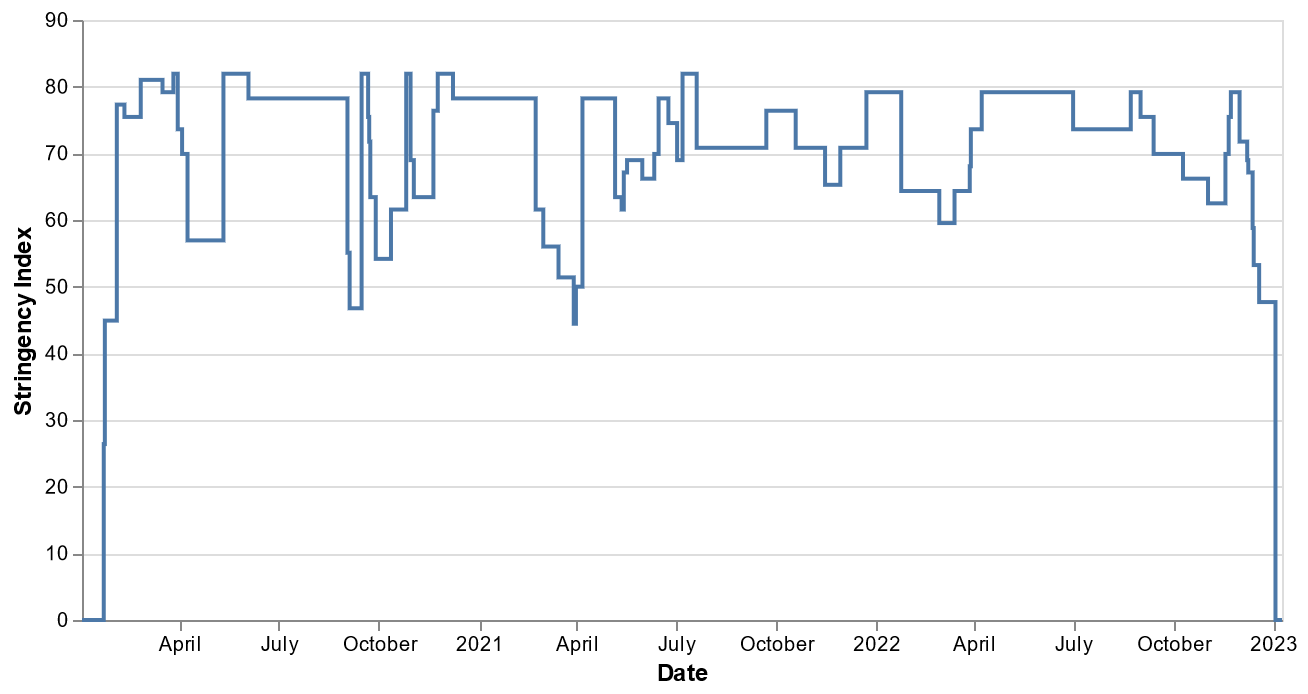
\includegraphics[scale=0.4]{graphics/stringency_line.png}

\end{center}

In addition to market data, we collect data within the same period on the Chinese government response to COVID-19 from the Oxford Covid-19 Government Response Tracker (OxCGRT), as produced by the Blavatnik School of Government at the University of Oxford \citep{OxCGRT}. In particular, we utilise the Stringency Index within our main specification, which seeks to record the severity of ‘lockdown style’ policies that primarily restricts people’s behaviour and movement.

\subsubsection*{[Methodology]}

We adopt the approach proposed by \citet{ch} (CH), utilising the relationship between dispersion and market returns as our measure of herding. However, we have chosen to utilise \citet{cck}'s (CCK) alternative specification, namely that our specification’s measure of dispersion is the cross-sectional absolute deviation (CSAD), expressed as

$$
CSAD_t=\frac{1}{N}\sum^N_{i=1}|R_{i,t}-R_{m,t}|
$$

where $N$ is the number of equities within our portfolio (being the CSI 300 as of 03/01/2020) $R_{i,t}$ is the observed stock return of equity $i$ at time $t$ and $R_{m,t}$ is the equally-weighted cross-sectional average of the $N$ returns within the portfolio. Following CCK, the foundation of our specification is

$$
CSAD_t=\gamma_0+\gamma_1 |R_{m,t}|+\gamma_2 R_{m,t}^2+\epsilon_t
$$

where $\gamma$ denote the model’s coefficients and $\epsilon_t$ the error term at time $t$. This model’s rationale is as follows: according to rational asset-pricing models, as individual assets have varying degrees of sensitivity to overall market return, the relationship between dispersions and market returns are linear and increasing. However, if herding is present within the market CCK suggests that this relationship will no longer hold, as investors’ conformity will result in a non-linear, decreasing or even negative relationship between the two variables. As such, if herding is present we would expect a negative $\gamma_2$, indicating a non-linear relationship. Conversely, in the absence of herding we would expect $\gamma_1$ to be positive and $\gamma_2$ to be insignificant.

$CSAD$ benefits from it’s ability to capture non-linear herding effects, in combination with the inclusion of $R_{m,t}^2$, that $CSSD$ is unable to capture, which CCK notes results in CH’s approach being overly strict. It is notable that, additionally, $SCSAD_t$ provides a better fit for our data compared to $CSSD_t$, which has been observed in prior literature \citep{gleason}. Whilst observers state concerns regarding $CSAD$’s construction, notably it’s reliance on proxying for unobservable variables within Black’s CAPM \citep{yao, tan}, the two measures share a correlation coefficient of $\rho=0.89$ within our sample and as such are expected to produce similar results. Additionally the model has high levels of structural multicollinearity regarding $R_{m,t}$ and $R_{m,t}^2$, which will reduce the efficiency of the model's standard errors. However, given OLS remains BLUE.

Following empirical consensus \citep{yao, tan, chiang} we utilise logarithmic daily returns within our calculations of $CSAD_t$ and $R_{m,t}$

$$
R_{i,t}=100\times(\ln{P_{i,t}}-\ln{P_{i,t-1}})
$$

where $P_{i,t}$ is the closing price of equity $i$ at time $t$. This is in order to preserve time-additivity and log-normality, in addition to aiding interpretation of our model’s predicted coefficients.

\subsubsection*{[Extension 1 - The Effect of 'Lockdown Style' Policies on Herding]}

In order to distil China’s containment policy response over time, we utilise OxCGRT’s ‘Stringency Index’. This index calculates a daily average of 9 ‘lockdown style’ policy indicators the database records: closing of schools and universities, closing of workplaces, cancelling of public events, limits on gatherings, closing of public transport, shelter-in-place orders, restrictions on internal city/region movements, restrictions on international travel and presence of COVID-19 public information campaigns. Importantly to China, policies that only apply to a particular region rather than nationally are weighted less within the final index. We chose a variation of this Stringency Index that is split based upon how these policies depend on vaccination status, with weightings applied according to the vaccination rate of the population:

$$
STRINGENCY_t=[(stringency_{v,t}*W_{v,t})+(stringency_{nv,t}*W_{nv,t}]/100
$$


where $STRINGENCY_t$ is our specification’s measure, $stringency_{v,t}$ is the index score for policies applying to vaccinated individuals at $t$, $stringency_{nv,t}$ the index score for non-vaccinated based policies, and $W_{v,t}$ and $W_{nv,t}$ are the percentage of the population vaccinated and not-vaccinated respectively. We chose this to more accurately reflect how containment policies apply to China’s population at a given time. We have re-scaled the stringency index from 0 to 1, compared to it's original form of 0 to 100, in order to aid interpretation of our estimated coefficients.

As highlighted by \citet{aknin}, many previous studies utilising ‘lockdown style’ policy regressors fail to control for confounding variables such as local infection and mortality rate. Not including these variables within our regression could result in an understatement within our $STRINGENCY_t$ coefficient given previous studies have suggested the pandemic results in lower herding behaviour within China (Wu et al., 2020). As such, our Model 1 takes the following form:

\begin{equation}\label{model-1}
CSAD_t=\gamma_0+\gamma_1 |R_{m,t}|+\gamma_2 R_{m,t}^2+\gamma_3STRINGENCY_t+\Gamma{A}+\epsilon_t
\end{equation}

where $A$ is a matrix of controls with the vector $\Gamma$ of coefficients. Formally, within our controls we include a 7 day moving average of the number of deaths, and the daily single-vaccination rate. A moving average has been chosen for our mortality rate measure in order to smooth measurement errors present in daily data.

This approach has limited power to capture the possible non-linear relationship between containment policies and mental health in herding. It may be that cognitive stress strong enough to effect herding only occurs during demonstrably limiting lockdown policies. We have included multiple alterations to Model 1 that seek to capture this non-linear relationship. Firstly, we have replaced $STRINGENCY_t$ with dummy indicators $S^{j\%}$, taking the value 1 if the Stringency Index value falls within the upper $j$th percentile of the index’s distribution. As such, our Model 2 is expressed as

\begin{equation}\label{model-2}
CSAD_t=\gamma_0+\gamma_1 |R_{m,t}|+\gamma_2 R_{m,t}^2+\gamma_3R_{m,t}^2*S^{j\%}+\Gamma{A}+\epsilon_t.
\end{equation}

We run regressions with an $S^{j\%}$ for the upper 25th, 10th and 5th percentile. This addition is constructed as an interaction term to capture effect severe lockdowns have on the relationship between $R^2_{m,t}$ and $CSAD_t$.

Secondly, following \citet{aknin} we also evaluate the possible cumulative effect of lockdown-style policies by including the variable $D_t$ within Model 3, taking on the number of days the population were under high-stringency policies:

\begin{equation}\label{model-3}
CSAD_t=\gamma_0+\gamma_1 |R_{m,t}|+\gamma_2 R_{m,t}^2+\gamma_3STRINGENCY_t+\gamma_4DAYS_t+\Gamma{A}+\epsilon_t
\end{equation}

where $DAYS_t$ is the cumulative number of days $STRINGENCY_t>70$, with the indicator resetting once the index drops below 70. We chose 70 as our threshold for high-stringency once again following Aknin.

\subsubsection*{[Extension 2 - Time Series Analysis]}

Our static model is likely subject to issues causing failure of the Gauss-Markov assumptions necessary to maintain efficiency of OLS as an estimator and validity of standard errors. 

Particularly, it is likely our error term suffers from serial correlation, as market dispersion measures such as CSAD and high-frequency market data in general are frequently observed to exhibit high levels of autocorrelation \citep{cck}. As such it is necessary we test for correlations between our model’s residuals over time in order to determine if the true disturbances are auto-correlated. Observing the partial autocorrelation function (PACF) we can see that autocorrelations of $CSSD$ are present for values of $t<10$, and as such it is appropriate to include lags until this point as to control for this residual correlation. The PACF partials out residual correlations of intervening lags between time periods, as such allowing us to observe the level of partial autocorrelation at each time period:

$$
PACF=\frac{cov(CSSD_t,CSSD_{t-j}|CSSD_{t-k}\in{t<k<j})}{\sqrt{var(CSSD_t|CSSD_{t-k}\in{t<k<j})var(CSSD_{t-j}|CSSD_{t-k}\in{t<k<j})}}
$$

These significant partial-correlations reject the null that our underlying process can be represented by a moving-average process of MA(0), and instead indicates that variation $CSSD_t$ is comprised of $CSSD$ values up to 10 days prior. We also investigate the possibility of our model’s estimated auto-regressive component actually being a unit root process, or a random-walk:

$$
CSSD_t=\rho{CSSD_{t-1}}+...+\epsilon_t
$$

with $\rho=1$. Such a highly persistent process fails the requirement of weak dependence and we will not be able to utilise the Ergodic Theorem nor the Central Limit Theorem necessary for coefficient estimation. As such it is prudent to run an Augmented \citet{dfuller} test, fitting the model above with an intercept. The test is augmented with lags of $\Delta{CSSD_t}$ in order to control for serially-correlated errors within the test’s model. Under the null the parameter for $CSSD_{t-1}$ is equal to 0, equivalent to $\rho=1$ above. As outlined by cite, statistical significance of coefficients from this regression can be determined using usual t tests and values.

We confirm the results of the PACF and Augmented Dickey-Fuller test by running a \citet{breusch} \citet{godfrey} test. This is necessary as, given the test utilises the Lagrange Multiplier (LM) statistic, we can conduct a joint test of higher autocorrelation up to a specified level of lags. The test, derived from constrained optimisation, is equivalent to running an OLS regression on a ‘restricted’ version of our model, or our model specification excluding any auto-correlated errors, to obtain predicted residuals $\hat{\epsilon}_t$ for all $t\in[0,n]$. $\hat{\epsilon}_t$ is then regressed upon the remaining predicted residuals and independent variables. It is worth noting that this test is beneficial above the Augmented Dickey-Fuller as the presence of our independent variables within the auxiliary regression means the strict-exogeneity assumption is no longer needed. The LM statistic is constructed:

$$
LM=(n-p)R^2_{\hat{\epsilon}} \sim\chi^2_p
$$

where $n$ is the number of observations, $p$ is the number of autocorrelations and $R^2_{\hat{\epsilon}}$ the R-squared of the auxiliary regression. This statistic, following a Chi-Squared distribution, tests the joint null that the coefficient of each level of autocorrelation is equal to 0.

In addition to autocorrelation, heteroskedastic errors within our model pose a threat to the efficiency of OLS as an estimator in addition to the validity of our usual standard errors.

To correct for these factors within our standard errors and ensure validity of inference tests, we chose to utilise the \citet{newey} estimator for our regressions in order to compute heteroskedastic and autocorrelative consistent (HAC) errors.

The Newey-West estimator extends the \citet{white} formulation, which builds upon the standard OLS variance estimator and produces heteroskedastic consistent errors by estimating the variance at each value of $t$ within our sample via $\hat{\epsilon}^2_tx_tx'_t$. The White estimator for can be expressed as $Var(\hat{\beta})=(X'X)^{-1}X'\hat{\Omega_0}X(X'X)^{-1}$, with:

$$
X'\hat{\Omega_0}X=\frac{1}{T}\sum_{t=1}^T\hat{\epsilon_t}^2x_t'x_t
$$

where $X$ is a $t\times1$ matrix of the vectors $x_t$ containing our independent variables at $t$, $\hat{\beta}$ is a matrix of the model’s predicted coefficients, $\hat{\epsilon_t}$ is the predicted residuals at $t$ and $\Omega_0$ is the variance-covariance matrix for our residuals under no serial correlation. When introducing the possibility of autocorrelation, the White formulation is no longer valid as the covariance values within the variance-covariance matrix can no longer assumed to be 0. Likewise, we cannot extend this White formulation to be $X'\hat{\Omega}X$, as given $\hat{\Omega}=\hat{\epsilon}\hat{\epsilon}'$, this estimator results in a $\widehat{Var(\hat{\beta})}=0$.

The Newey-West estimator proposes a solution to this applying a weighting of $w_l=1-\frac{l}{L+1}$ to each autocorrelation within the variance-covariance matrix according to their level of autocorrelation, $L$. As such, the Newey-West variance estimator is expressed by

$$
\widehat{Var_{nw}(\hat{\beta})}=(X'X)^{-1}X'\hat{\Omega}_{nw}X(X'X)^{-1}=X'\hat{\Omega}_0X+\frac{1}{T}\sum^L_{l=1}\sum^T_{t=l+1}w_l\epsilon_t\epsilon_{t-l}(x_tx'_{t-l}+x_{t-l}x'_t)
$$

Autocorrelations further away from $t$ are weighted less within our estimator, which converge to 0 under the assumption of weak-dependence, maintaining efficiency of the estimator by preventing too many estimations of coefficients.

In order to calculate how many levels of autocorrelations we take into account, i.e. our truncation parameter $L$, we observe both common practice outlined in \cite{greene}, dictating that $L\approx{T^{1/4}}$, and the results of our PACF.


\subsection{Empirical Analysis and Results}

\begin{table}[!htbp]
    \caption{Summary statistics} \label{tab:table1}
    \centering
    {
\def\sym#1{\ifmmode^{#1}\else\(^{#1}\)\fi}
\begin{tabular}{l*{1}{cccccc}}
\toprule
                    &         Sum&        Mean&          SD&         Min&         Max&           N\\
\midrule
CSAD                &       1,110&      1.5165&      0.3596&      0.7321&      2.9229&         732\\
CSSD                &          93&      0.1276&      0.0288&      0.0592&      0.2505&         732\\
Absolute Market Return&         637&      0.8705&      0.8728&      0.0011&      8.9773&         732\\
Market Return Squared&       1,112&      1.5186&      4.1696&      0.0000&     80.5914&         732\\
Stringency Index    &         511&      0.6983&      0.1417&      0.0000&      0.8194&         732\\
Shelter in Place Indicator&       1,771&      2.4194&      0.9604&      0.0000&      3.0000&         732\\
Vaccination Rate    &      28,667&     39.1630&     42.2270&      0.0000&     89.3500&         732\\
COVID-19 Deaths 7-Day Rolling Average&      44,556&     60.8692&    291.1154&      0.0000&     4.0e+03&         732\\
COVID-19 Daily Cases&    66215455&     9.0e+04&     5.9e+05&      0.0000&     7.0e+06&         732\\
\bottomrule
\end{tabular}
}

\end{table}

\begin{table}[htbp]\small \centering
\begin{threeparttable}
\def\sym#1{\ifmmode^{#1}\else\(^{#1}\)\fi}
\caption{Regression Results \label{reg1}}
\begin{tabular}{l*{6}{c}}
\toprule
                    &\multicolumn{1}{c}{(A)}         &\multicolumn{1}{c}{(B)}         &\multicolumn{1}{c}{(C)}         &\multicolumn{1}{c}{(D)}         &\multicolumn{1}{c}{(E)}         &\multicolumn{1}{c}{(F)}         \\
\midrule
$|R_{m,t}|$&     0.18341\sym{***}&     0.18214\sym{***}&     0.16315\sym{***}&     0.18059\sym{***}&     0.19307\sym{***}&     0.18281\sym{***}\\
                    &   (0.02499)         &   (0.02437)         &   (0.02413)         &   (0.02464)         &   (0.02424)         &   (0.02444)         \\
\addlinespace
$(R_{m,t}-\bar{R_m})^2$&    -0.00936\sym{**} &    -0.00998\sym{**} &    -0.01077\sym{***}&    -0.00954\sym{**} &    -0.01095\sym{**} &    -0.01009\sym{**} \\
                    &   (0.00462)         &   (0.00470)         &   (0.00321)         &   (0.00462)         &   (0.00460)         &   (0.00476)         \\
\addlinespace
$STRINGENCY_t$    &                     &     0.42265\sym{**} &                     &                     &                     &                     \\
                    &                     &   (0.21290)         &                     &                     &                     &                     \\
\addlinespace
$S_t^{0.25}\times{(R_{m,t}-\bar{R_m})^2}$&                     &                     &     0.01377\sym{***}&                     &                     &                     \\
                    &                     &                     &   (0.00518)         &                     &                     &                     \\
\addlinespace
$S_t^{0.10}\times{(R_{m,t}-\bar{R_m})^2}$&                     &                     &                     &     0.00186         &                     &                     \\
                    &                     &                     &                     &   (0.00776)         &                     &                     \\
\addlinespace
$S_t^{0.05}\times{(R_{m,t}-\bar{R_m})^2}$&                     &                     &                     &                     &    -0.10850\sym{***}&                     \\
                    &                     &                     &                     &                     &   (0.03308)         &                     \\
\addlinespace
$LOCKDOWN_t$&                     &                     &                     &                     &                     &     0.04907\sym{*}  \\
                    &                     &                     &                     &                     &                     &   (0.02613)         \\
\addlinespace
$DAYS_t$                &                     &                     &                     &                     &                     &    -0.00055         \\
                    &                     &                     &                     &                     &                     &   (0.00065)         \\
\addlinespace
Vaccination Rate    &                     &    -0.00149\sym{***}&    -0.00139\sym{***}&    -0.00144\sym{***}&    -0.00155\sym{***}&    -0.00129\sym{**} \\
                    &                     &   (0.00054)         &   (0.00054)         &   (0.00054)         &   (0.00054)         &   (0.00063)         \\
\addlinespace
COVID-19 Deaths&                     &    -0.00035\sym{***}&    -0.00044\sym{***}&    -0.00045\sym{***}&    -0.00046\sym{***}&    -0.00036\sym{***}\\
                    &                     &   (0.00013)         &   (0.00012)         &   (0.00012)         &   (0.00012)         &   (0.00012)         \\
\addlinespace
Constant            &     1.37724\sym{***}&     1.14927\sym{***}&     1.45928\sym{***}&     1.45403\sym{***}&     1.45549\sym{***}&     1.34074\sym{***}\\
                    &   (0.02616)         &   (0.15211)         &   (0.03365)         &   (0.03340)         &   (0.03411)         &   (0.06409)         \\
\midrule
Adjusted $R^2$        &         0.1277         &         0.1935         &         0.1892         &         0.1833         &         0.1966         &         0.1916         \\
\bottomrule
\end{tabular}
\begin{tablenotes}
\footnotesize Standard errors in parentheses and based on Newey and West (1987)'s heteroscedasticity and autocorrelation consistent standard errors. This table reports the estimated coefficients and adjusted $R^2$ for the models defined in Section 3.1. Panel A contains results for the base model defined in Equation \ref{model-1}: $CSAD_t=\gamma_0+\gamma_1 |R_{m,t}|+\gamma_2 (R_{m,t}-\bar{R_m})^2+\epsilon_t$. Panel B contains results for the lockdown-policy extension model defined in Equation \ref{model-2}: $CSAD_t=\gamma_0+\gamma_1 |R_{m,t}|+\gamma_2(R_{m,t}-\bar{R_m})^2+\gamma_3STRINGENCY_t+\Gamma{A}+\epsilon_t$. Panels C D \& E contain results for the model defined in equation \ref{model-3}: $CSAD_t=\gamma_0+\gamma_1 |R_{m,t}|+\gamma_2 (R_{m,t}-\bar{R_m})^2+\gamma_3(R_{m,t}-\bar{R_m})^2*S_t^{j\%}+\Gamma{A}+\epsilon_t$ for the top 25th, 10th and 5th percentile respectively. Panel F contains the results for the model defined in Equation \ref{model-4}: $CSAD_t=\gamma_0+\gamma_1 |R_{m,t}|+\gamma_2 (R_{m,t}-\bar{R_m})^2+\gamma_3LOCKDOWN_t+\gamma_4DAYS_t+\Gamma{A}+\epsilon_t$.\\
\sym{*} \(p<0.10\), \sym{**} \(p<0.05\), \sym{***} \(p<0.01\)\\
\end{tablenotes}
\end{threeparttable}
\end{table}


\break

\section{Conclusion}

\break

\section{Appendix}

\begin{singlespace}

    \bibliographystyle{authordate1}
    \bibliography{TeX_files/bibliography}
    \addcontentsline{toc}{subsection}{5.0 \hspace{0.25cm} References}
    
    \break
    
    \markdownInput{TeX_files/AED_codebook.md}
    
\end{singlespace}

\end{document}
